Att exekvera ett program symboliskt innebär att representera värden utefter 
programflödet som symboliska restriktioner, vilka kan lösas av automatiserade 
teoremlösare (\emph{SMT solver}). En symbolisk körning representerar flera konkreta 
körningar eftersom de (symboliska) värden som används representerar grupper av 
konkreta värden vilka har gemensamt hur de påverkar programmets flöde. 

Vägar i programmets kontrollflöde utforskas med symboliska uttryck för de 
begränsningar som finns på programmets variabler -- vilka egenskaper de måste uppnå 
för att just denna väg ska kunna följas. Eftersom de symboliska värdena har kapacitet 
att representera grupperingar av konkreta värden istället för enskilda sådana, 
utförs en generaliserad testning av programmet, som ger insikt i hur programmet 
beteer sig givet en grupp av parametrar som alla på grund av någon eller några 
gemensamma egenskaper, orsakar gemensamma beteenden i programmet. 

En symbolisk exekveringsmotor arbetar genom att först representera programmets input 
som symboliska variablar, vilka vid starten inte har några begränsningar, och när 
programflödet når en branch som baseras på någon av de symboliska variablerna, 
så väljer motorn en gren och tillsätter den grenens restriktioner på den symboliska 
variabeln för alla vägar som fortsätter utefter branchen. Operationer på värden 
under körningens väg översätts till symboliska operationer på motsvarande symboliska 
variabler. \cite{klee} När körning utefter grenen är slutförd så kan motorn börja om 
vid branchen och utforska andra alternativ med samma metodik. De tillståndsvillkor 
som en viss väg visas ha byggs därför successivt upp genom att motorn utökar de 
symboliska variablerna till villkorliga uttryck allt eftersom vägen följs. 

De fel som hittas genom symbolisk exekvering är tillförlitliga då metoden ej ger falskt 
positiva resultat. Huruvida villkorsblock av program är nårbara kan evalueras med 
säkerhet eftersom de krav som måste uppfyllas för att följa vägen dit dokumenteras under 
den symboliska körningen, och resulterar i fullständiga symboliska representationer 
som en automatiserad teoremlösare (SMT solver) kan appliceras på. 

Symbolisk exekvering är användbart för att resonera kring hur programmet beter sig 
beroende på grupperingar av input. För program där få värden tar gemensamma vägar blir 
fördelen över att istället använda dynamisk testning av konkret data dock låg. 

Eftersom symbolisk exekvering kan leda till \emph{path explosion} är det inte effektivt 
att alltid undersöka alla branchar i ett program. Exempel på metoder för att undvika 
path explosion är \emph{state-merging} och \emph{heuristics}. 

\begin{figure}[H]
\centering
\begin{lstlisting}[label={list:first}, language=Python, frame=single]
x = int(argv[1])
y = int(argv[2])
z = 2 * y

if x == 100000: 
    if x < z:
        // fabricated scenario of 
        // memory vulnerability
        error_leading_to_mem_vuln()
    else:
        run_other_important_code()
else:
    run_important_code()

\end{lstlisting}
\caption{}
\end{figure}

\begin{figure}[H]
\centering
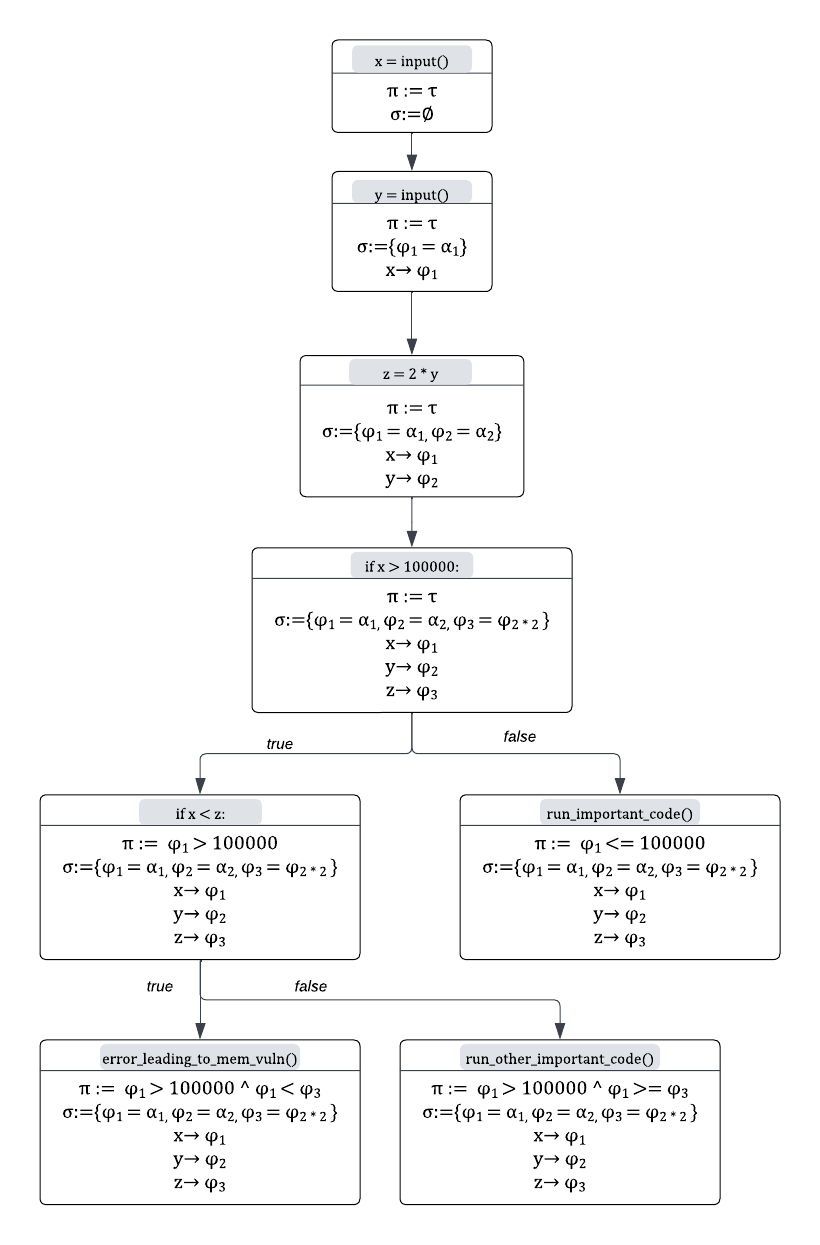
\includegraphics[scale=0.5]{figures/final_symbolic_example_graph.png}
\caption{Concolic testning av enkel exempelkod}
\end{figure}


